\documentclass[journal,12pt,onecolumn]{IEEEtran}
\usepackage{cite}
\usepackage{caption}
\usepackage{graphicx}
\usepackage{amsmath,amssymb,amsfonts,amsthm}
\usepackage{algorithmic}
\usepackage{graphicx}
\usepackage{textcomp}
\usepackage{xcolor}
\usepackage{txfonts}
\usepackage{listings}
\usepackage{enumitem}
\usepackage{mathtools}
\usepackage{gensymb}
\usepackage{comment}
\usepackage[breaklinks=true]{hyperref}
\usepackage{tkz-euclide} 
\usepackage{listings}
\usepackage{gvv}
\usepackage[latin1]{inputenc} 
\usetikzlibrary{arrows.meta, positioning}
\usepackage{xparse}
\usepackage{color}                                            
\usepackage{array}                                            
\usepackage{longtable}                                        
\usepackage{calc}                                             
\usepackage{multirow}
\usepackage{multicol}
\usepackage{hhline}                                           
\usepackage{ifthen}                                           
\usepackage{lscape}
\usepackage{tabularx}
\usepackage{array}
\usepackage{float}

\usepackage{float}
\theoremstyle{remark}
\usepackage{circuitikz}
\captionsetup{justification=centering}
\usepackage{tikz}

\title{Matrices in Geometry 7.4.42}
\author{EE25BTECH11035 - Kushal B N}
\begin{document}
\vspace{3cm}
\maketitle
{\let\newpage\relax\maketitle}

\textbf{Question: }\\
Find the intervals of values of $a$ for which the line $y+x = 0$ bisects two chords drawn from a point $\brak{\frac{1+\sqrt{2}a}{2},\frac{1-\sqrt{2}a}{2}}$ to the circle $2x^2 + 2y^2 - (1+\sqrt{2}a)x - (1-\sqrt{2}a)y = 0$.

\vspace{0.5cm}

\textbf{Given: } \\
Circle C: $x^2 + y^2 - \frac{1+\sqrt{2}a}{2}x - \frac{1-\sqrt{2}a}{2}y = 0$\\
Point $\vec{P} = \myvec{\frac{1+\sqrt{2}a}{2}\\\frac{1-\sqrt{2}a}{2}}$\\
Line L: $\vec{n}_L^{\top}\vec{x} = 0$, where $\vec{n}_L = \myvec{1\\1}$

\vspace{0.5cm}

\textbf{Solution: }\\
The center of the circle is 
\begin{equation}
\vec{c} = \frac{1}{4}\myvec{1+\sqrt{2}a\\1-\sqrt{2}a}
\end{equation}
    
By observation,
\begin{equation}
    \vec{P} = 2\vec{c}
\end{equation}
The locus of midpoints, $\vec{M}$, of chords from $\vec{P}$ is given by,
\begin{equation}
    (\vec{M}-\vec{c})^{\top}(\vec{P}-\vec{M}) = 0
    \label{eq3}
\end{equation}
The midpoint $\vec{M}$ lies on the line L, the direction vector of which is
\begin{equation}
    \vec{m}_L = \myvec{1\\-1}
\end{equation}

\begin{equation}
\implies \vec{M} = \lambda\vec{m}_L
\end{equation}
Substituting this into equation \eqref{eq3}, we get
\begin{equation}
    (\lambda\vec{m}_L-\vec{c})^{\top}(\vec{P}-\lambda\vec{m}_L) = 0
\end{equation}
\begin{equation}
    \implies (\vec{m}_L^{\top}\vec{m}_L)\lambda^2 - \vec{m}_L^{\top}(\vec{P}+\vec{c})\lambda + \vec{c}^{\top}\vec{P} = 0
\end{equation}
For two distinct chords, the discriminant $\Delta = b^2 - 4ac > 0$.
\begin{equation}
    \Delta = \brak{\vec{m}_L^{\top}(\vec{P}+\vec{c})}^2 - 4\brak{\vec{m}_L^{\top}\vec{m}_L}\brak{\vec{c}^{\top}\vec{P}} > 0 \label{eq8}
\end{equation}
Here,
\begin{equation}
    \vec{m}_L^{\top}\vec{m}_L = \myvec{1&-1}\myvec{1\\-1} = 2
\end{equation}
\begin{equation}
    \vec{m}_L^{\top}(\vec{P}+\vec{c}) = \vec{m}_L^{\top}(3\vec{c}) = 3\myvec{1&-1}\frac{1}{4}\myvec{1+\sqrt{2}a\\1-\sqrt{2}a} = \frac{3\sqrt{2}a}{2}
\end{equation}
\begin{equation}
    \vec{c}^{\top}\vec{P} = 2\|\vec{c}\|^2 = \frac{1+2a^2}{4}
\end{equation}
Substituting into the inequality \eqref{eq8}:
\begin{equation}
    \brak{\frac{3\sqrt{2}a}{2}}^2 - 4(2)\brak{\frac{1+2a^2}{4}} > 0
\end{equation}
\begin{equation}
    \frac{9a^2}{2} - 2(1+2a^2) > 0
\end{equation}
\begin{equation}
    \frac{a^2}{2} > 2 \implies a^2 > 4
\end{equation}
\begin{equation}
    \implies a > 2 \quad \text{or} \quad a < -2
\end{equation}

\vspace{0.5cm}

\textbf{Final Answer: }\\
The intervals of values for $a$ are $(-\infty, -2) \cup (2, \infty)$.
\begin{equation}
    \fbox{$a \in (-\infty, -2) \cup (2, \infty)$}
\end{equation}

\begin{figure}[H]
    \centering
    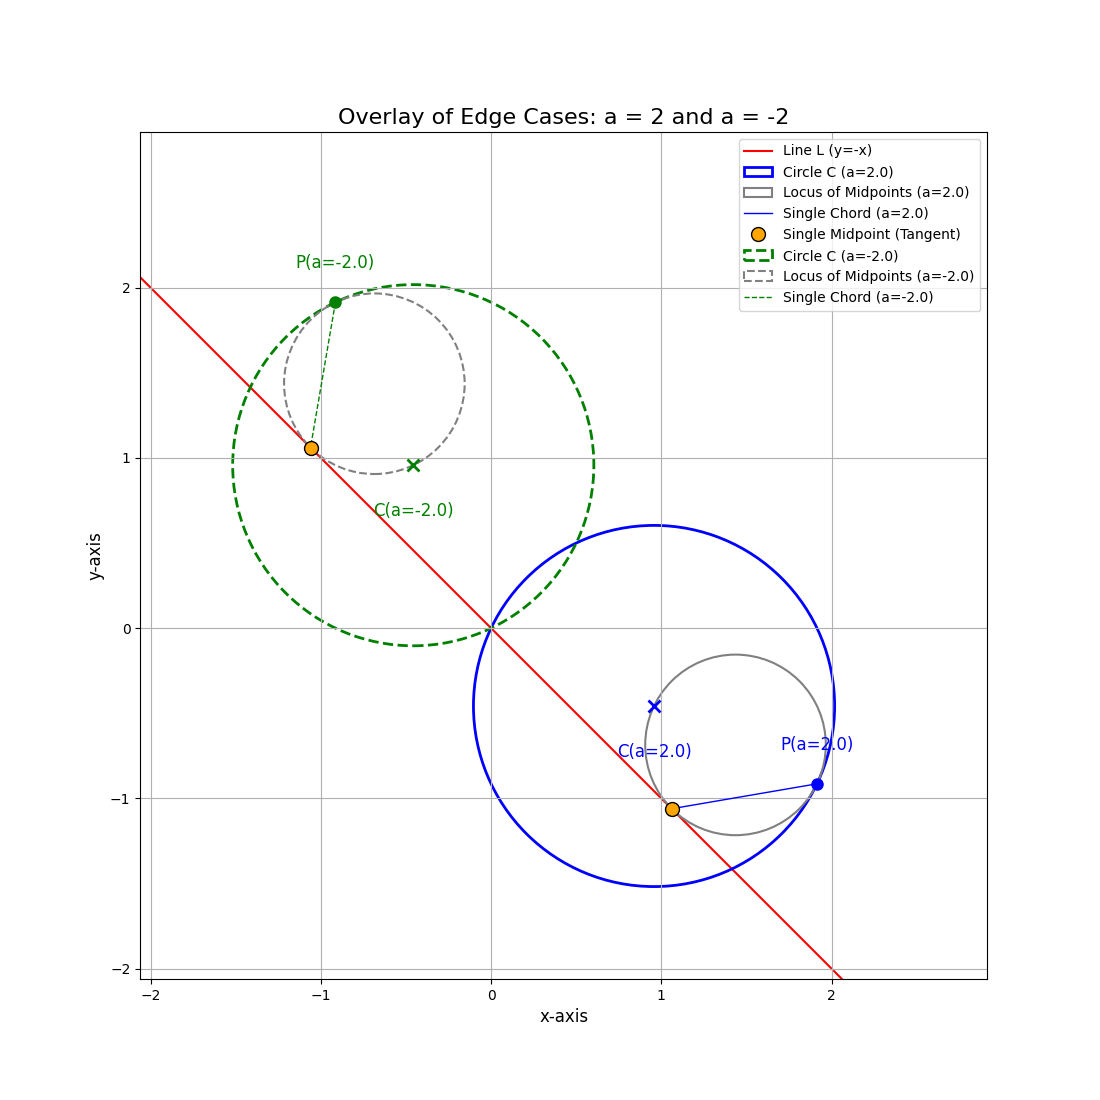
\includegraphics[width=0.75\columnwidth]{figs/fig.png}
    \caption{Plot for 7.4.42}
\end{figure}

\end{document}
